\documentclass{article}
\usepackage[utf8]{inputenc}
\usepackage[margin=.9in]{geometry}
\usepackage{siunitx}
\usepackage{graphicx}
\usepackage{placeins}
\usepackage{tipa}
\usepackage{float}
\usepackage{fancyhdr}
\usepackage{amsmath}
\usepackage{biblatex}
\usepackage{xcolor}
\usepackage{dirtree}
\usepackage[spanish]{babel}

\newcommand\myicon[1]{{\color{#1}\rule{2ex}{2ex}}}
% If you have actual icon images, use \includegraphics to include them
% If you are generating them, put in the appropriate code for them here
% now we make a command for a folder/file which inserts the icon and its label
% adjust this as needed. If you only have 2 icons, then you could create
% a \myfile and \myfolder command with the icon fixed.
\newcommand{\myfolder}[2]{\myicon{#1}\ {#2}}

\pagestyle{fancy}
\fancyhf{}
\rhead{Agustín Barrachina y Matias Dwek}
\lhead{Procesamiento de Voz: TP Final}
\rfoot{Page \thepage}

\title{%
  \LARGE Procesamiento de Voz \\
  \vspace{.3cm}
  \huge TP Final}
\author{\textbf{Agustín Barrachina y Matias Dwek}}
\date{\today}

\bibliography{references.bib}

\begin{document}

\maketitle

\part*{Primera Entrega: Detección por LPC}

\subsection*{Estructura del proyecto}

El proyecto se divide en varias carpetas con la siguiente estructura: \\


% TODO: no me gusta el formato éste, hay que ver si hay una forma mejor de hacer ésto.
\dirtree{%
.1 \myfolder{red}{LipSync}.
.2 \myfolder{blue}{images}.
.3 \myfolder{blue}{icons}.
.3 \myfolder{blue}{mouth types}.
.2 \myfolder{blue}{out}.
.2 \myfolder{blue}{sounds}.
.2 \myfolder{blue}{src}.
.3 \myfolder{yellow}{main.py}.
.3 \myfolder{yellow}{data.py}.
.3 \myfolder{yellow}{central widget.py}.
.3 \myfolder{yellow}{process.py}.
.3 \myfolder{yellow}{processing functions.py}.
.3 \myfolder{yellow}{pvutils.py}.
}

\vspace{.5cm}

La carpeta \textit{images} guarda las imágenes que utilizará el programa. \textit{out} puede ser utilizada para guardar los archivos dat exportados por el programa. Para una explicación sobre la extensión de dicho archivo referirse a la sección \ref{sec:dat}. \textit{sounds} posee archivos de audio wav que pueden usarse como ejemplos con el programa. Finalmente, en  \textit{src} se encuentran todos los archivos que poseen el código del programa. Cada archivo posee una explicación comentada con lo cual se omitirá la explicación de cada uno en particular salvo por algunos detalles que se consideran importantes remarcar.

\textit{data} posee una clase \textit{singleton} la cual se utiliza para compartir la información principal de todo el programa como ser el archivo de audio wav sobre el cual trabajar. La estrategia singleton resulta particularmente útil para casos como éste programa ya que se evita de ésta forma el pasaje de parámetros básicos como la frecuencia de sampleo.

El archivo \textit{main.py} posee una clase denominada \textit{App} la cual se encarga del control principal del principal del programa.
        
\subsubsection*{extensión dat} \label{sec:dat}

Dicho archivo posee información sobre los fonemas que se encuentran en cierto audio.
Cada línea del archivo posee un número seguido por un texto. El número indica que a partir de dicha muestra, el audio posee un fonema el cual se corresponde con el texto que le sigue, hasta el fin del archivo de audio o hasta que una nueva línea indique que hay un nuevo fonema.

% TODO: poner un ejemplo para clarificar.

\subsection*{Graphic User Interfase y funcionalidades}

Se implementó una GUI en Python que permite cargar un audio y separarlo en los diferentes fonemas vocales. Una vez aplicado el procesamiento de identificación de fonemas, en la reproducción una representación de boca seguirá las posiciones correspondientes al audio.

En la siguiente figura puede verse una imagen de la forma general del programa:

\begin{figure}[H]
	\centering
	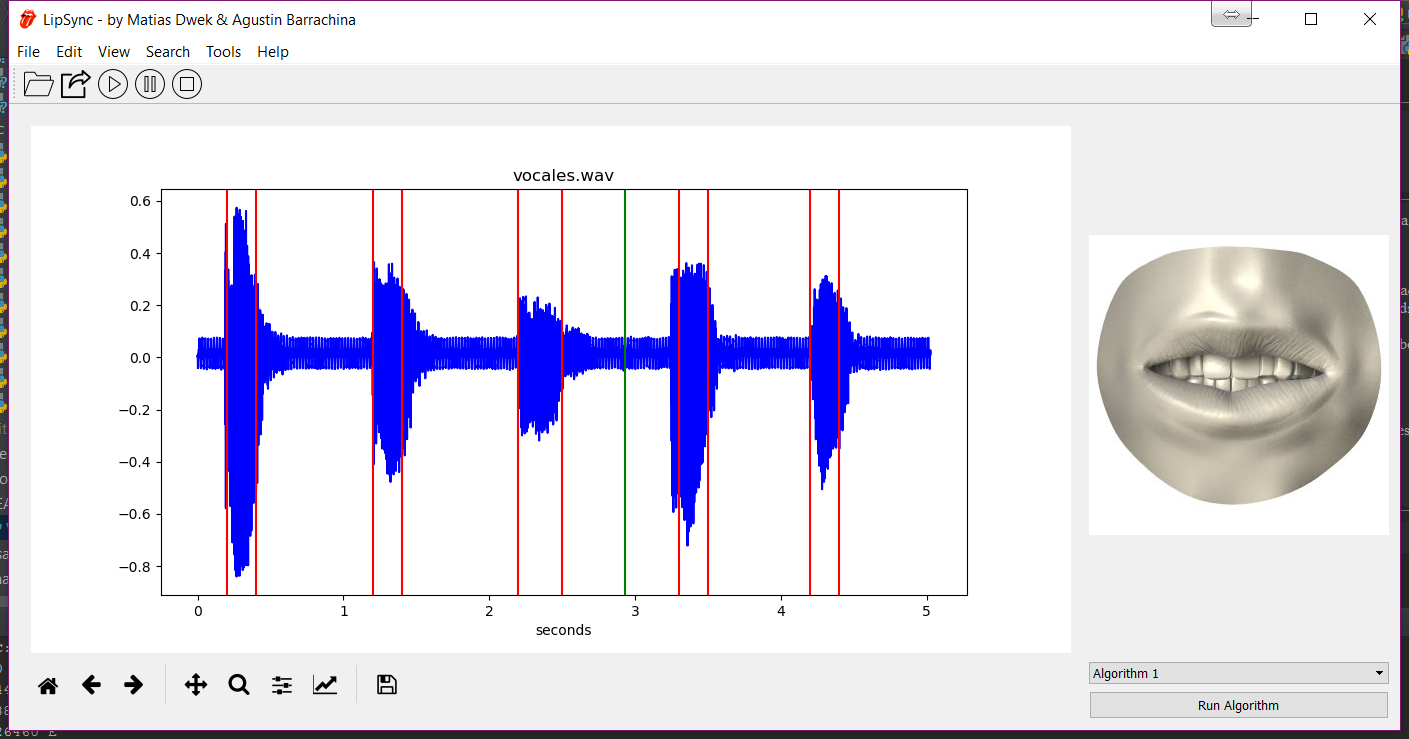
\includegraphics[width=15cm]{programa.png}
	\caption{GUI}
	\label{fig_gui}
\end{figure}

El programa posee un menú con la siguiente estructura:

\begin{itemize}
  \item File
  \begin{itemize}
      \item Open (Ctrl+O): Abre un archivo wav. Al activar la opción se abre un explorador de carpetas cuya ubicación por defectos en la carpeta sounds. El explorador permite únicamente seleccionar archivos wav.
      \item Export (Ctrl+E): Exporta el resultado del algoritmo de detección de fonemas en un archivo con extensión dat. Ésta acción abre un explorador de archivos al igual que la opción <<Open>>
      \item Quit (Ctrl+Q): Cierra el programa.
  \end{itemize}
  \item Edit
  \item View: En un futuro se planea implementar la opción de agregar o eliminar toolbars para una visualización más dinámica.
  \item Search
  \item Tools
  \item Help
\end{itemize}

Como se puede ver, algunas opciones del menú poseen un shortcut para poder activar la opción con una combinación de teclas, como por ejemplo usar \texttt{Ctrl+O} para abrir. 

El programa posee una <<toolbar>> la cual contiene iconos que permiten hacer las mismas opciones que <<Open>> y <<Export>> mencionadas anteriormente. Además posee teclas de <<Play>>, <<Stop>> y <<Pause>> que no se activan hasta que el programa haya abierto algún archivo wav. Las mismas permiten reproducir dicho audio y detenerlo. Sin embargo la opción de pausa no realiza acción en ésta versión de la entrega.

El programa posee finalmente una sección (Widget) principal o central en donde se encuentran los demás elementos de la GUI.

Dicho widget se posee un diseño horizontal (mediante la función QHBoxLayout de PyQt5). Dicho diseño organiza los elementos de forma horizontal, de izquierda a derecha. Como solo hay dos elementos lo dividiremos en el elemento de la izquierda y el elemento de la derecha.

El elemento de la izquierda posee una figura en la cual se gráfica la señal de audio (si efectivamente hay alguna señal cargada). Si los fonemas fueron detectados, se marca con lineas verticales rojas el lugar del comienzo de cada fonema omitiendo el primer fonema (ya que sería una linea vertical en el tiempo 0 por ser el fonema inicial y se consideró que no era gráficamente amigable).

Debajo del gráfico hay una barra de herramientas que permite modificar varias propiedades del gráfico y realizar otras opciones como hacer zoom, guardar la imagen, cambiar los ejes, etc.

El elemento de la derecha se encuentra a su vez organizado de forma vertical (función QVBoxLayout de PyQt5). La misma posee una imagen que mostrará una foto de la forma de la boca según el fonema que se esté reproduciendo. En la versión de la entrega hubo un problema que no cambiaba la imagen en paralelo con la reproducción del audio sino que sólo actualizaba una vez que el audio terminada de reproducirse. Dicho problema ya fue resuelto y se explica en la sección \ref{sec:nuevas-mejoras}.

Debajo de la imagen aparece un <<drop down list>> donde figuran los distintos algoritmos posibles para calcular la ubicación de los fonemas. Como en la entrega solo se aplicó un algoritmo, dicha lista no realiza acción alguna en el programa actual. Simplemente se coloca a modo de ejemplo.

Finalmente se encuentra un botón que permite correr el algoritmo seleccionado en el <<drop down list>> inmediatamente superior al mismo y que calcula la ubicación de los fonemas. Es importante destacar que sin correr previamente el algoritmo con dicho botón, al reproducir el audio no se mostrará las imágenes de la boca de forma correcta.

\subsection*{Identificación de fonemas vocales}

En esta primera versión del TP se implementó la identificación de fonemas vocales. Esta se realiza a partir de un análisis por LPC y de la detección de los formantes de cada fonema. El análisis de la señal se realiza por frames, de aproximadamente \SI{20}{ms} y se procesa cada frame con una ventana de Hann con un overlap del 50\%. En una primera parte se identifica qué partes del audio son silencio y qué partes son voz a partir de la energía de cada frame, con la función \texttt{short\_time\_energy()}. Una vez esto realizada, se calculan los coeficientes LPC de cada frame. A partir de estos se estima la envolvente espectral de la señal y, siguiendo los criterios establecidos en \cite{snell1993formant} y en \cite{mathworks1}, conservamos los formantes con frecuencias superiores a \SI{90}{Hz} con ancho de banda menor a \SI{400}{HZ}. En la figura \ref{fig_estimacion} se puede observar el resultado de esta estimación para un frame con el fonema /a/. Si se toman los dos máximos que cumplen con los criterios enunciados, encontramos que el primer formante se encuentra \SI{853}{Hz} y el segundo en \SI{1807}{Hz}, lo que efectivamente corresponde al fonema /a/.

\begin{figure}[H]
	\centering
	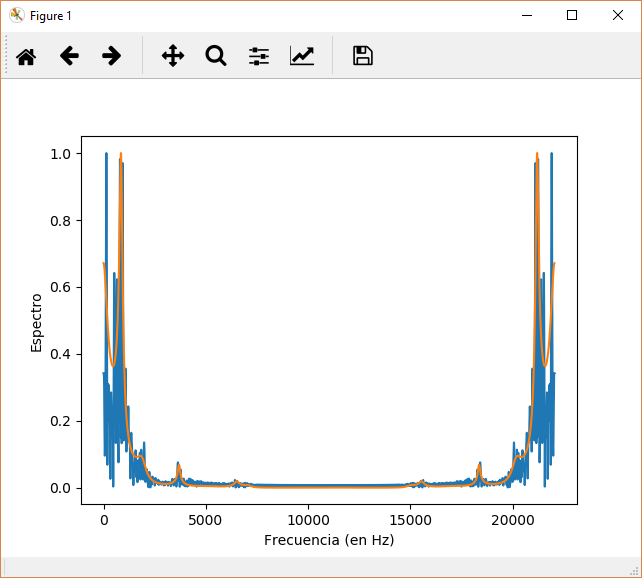
\includegraphics[width=15cm]{estimacion_LPC.PNG}
	\caption{Resultado de la estimación de la envolvente espectral para el fonema /a/}
	\label{fig_estimacion}
\end{figure}
 

Una vez calculados los formantes, se pasa a una etapa de decisión en la que se normalizan los resultados encontrados respecto al máximo valor de frecuencia posible para un formante determinado y se calcula qué fonema minimiza la distancia cuadrática. Se utilizan dos formantes de referencia para cada fonema.

Finalmente, para no tener en cuenta la mala estimación de un solo frame, se busca el fonema más común dentro de un rango de \SI{50}{ms}, teniendo en cuenta las duraciones de los fonemas vocales como se establecen en \cite{kuwabara1996acoustic}.
 

\section*{Nuevas modificaciones} \label{sec:nuevas-mejoras}

Se agregó una linea vertical verde que marca en tiempo real el momento del audio en reproducción.

Se corrigió el bug de la imágen de la boca de forma que en éste momento ya muestra en tiempo real la boca equivalente al fonema que se está reproduciendo.
El problema ocurría porque el loop donde cambiaba las imágenes no devolvía el control a la GUI principal para que refrescara la pantalla. Al aplicar ésto permitió poder detener el audio en reproducción ya que en la versión anterior el botón solo andaba si no se refrescaba las imágenes.

\section*{Trabajo futuro}

Para la entrega final agregaremos la predicción del resto de los fonemas e incluiremos métodos alternativos al de LPC. Además, incluiremos la opción de ajustar los diferentes parámetros de los algoritmos, como tamaño del frame, tipo de ventana, ... Además se agregará la funcionalidad de modificación de la  duración de la señal, del filtro de cavidades y de la frecuencia de los pulsos glotales.

\part*{Segunda Entrega: RNN-LMST}

Se aplicó un algoritmo de reconocimiento de voz basado en el trabajo de \cite{RNN_HINTON}. En el mismo se realizó una red neuronal recursiva para lograr la detección de fonemas. Las redes neuronales recursivas (RNN) son redes neuronales en las que las conexiones entre los nodos presentan ciclos, lo que permite la simulación de una variación dinámica del tiempo, característica particularmente atractiva para trabajar con el procesamiento de voz. A diferencia de las Deep Neural Networks (DNN), que trabajan con una ventana corrediza de tamaño fijo, las RNN pueden trabajar con contextos que varían dinámicamente, como por ejemplo el cambio de la velocidad de hablan entre dos locutores distintos. Esto se logra a partir de la recursividad de la red, a través de la realimentación proveniente de de ciclos anteriores. Las activaciones se almacenan en los estados internos de la red y permiten a la misma adquirir la capacidad de trabajar con memoria de la información contextual de la señal \cite{sak2014long}. Además, se trabajó con una arquitectura Long short-term memory (LSTM), que es un tipo particular de RNN, que contiene unidades de memoria en la \textit{hidden layer} recursiva que le permiten a la red aprender dependencias de largo plazo, característica en la que las RNN no resultan efectivas. Es por esto que este método se utiliza en el área del procesamiento de voz.


Para entrenar la red se utilizó una base de datos obtenida en \cite{LDC}.

\subsection*{Procedimiento}

El primer paso fue parsear los datos. Para iniciar se modifican los datos para que tengan media cero y varianza unitaria.

En el trabajo de \cite{RNN_HINTON} utilizan 40 coeficientes MFCC (Mel-Frequency Cepstral Coeficients) con sus respectivos delta y delta-delta. Sin embargo, con el objetivo de ahorrar tiempo y espacio se utilizaron solo 13 MFCC ya que son las que contienen mayor cantidad de información. Usar más (por ejemplo 26) duplicaría el tamaño de los archivos que con solo 13 coeficientes pesan más de 1.5 GB. 

Se usaron 3 capas ocultas Y 250 celdas de LSTM para la red ya que ésta fue la configuración que mejor resultado dio según \cite{RNN_HINTON}. 

Si bien \cite{RNN_HINTON} utiliza un optimizador de sgd, en nuestro caso se usó un optimizador Adam \cite{ADAM} ya que  experimentalmente pareció dar mejores resultados (si bien no se realizó una verificación exhaustiva). Siendo \cite{ADAM} más reciente que el trabajo \cite{RNN_HINTON}, explicaría porqué no se usó ese optimizador en el trabajo en cuestión. 

El trabajo a su vez utilizó una función de pérdida CTC (Connectionist Temporal Classification), sin embargo por una dificultad en la librería utilizada para aplcar dicha función, se utilizó directamente la \textit{categorical crossentropy}

\subsection*{Resultados}

Se alcanzó una performance de casi el 80\% (si bien en \cite{RNN_HINTON} se logra sobrepasar este valor, en la misma utilizan 120 epochs mientras que en nuestro caso no se pudo superar las 20, entre otros factores que pueden afectar el resultado. Sin embargo, éste número no es tan satisfactorio, tener una eficiencia del 80\% significa que un fonema de cada 5 va a estar errado, lo cual introduce mucho error y genera un archivo en donde los fonemas cambian casi constantemente según la longitud de las ventanas utilizadas (en nuestro caso 0.01 segundos).

Se aplicó entonces un filtro pasa bajos en donde se eliminaban mediante cierta técnica la cantidad de fonemas equívocos. Basados en el siguiente criterio: \textit{Un error no se repetirá de forma prolongada en el tiempo}. Con dicha lógica se buscó implementar un algoritmo que elimine los casos de fonemas aislados con duración corta. Sin embargo, en casos donde el error ocurra en cercanía con el reciente cambio de fonema. Ésta lógica podría eliminar el fonema correcto. Es para reducir la probabilidad de estos casos que se implementó un algoritmo recursivo que primero elimina fonemas de una sola ventana de duración, y va aumentando la cantidad de ventanas con cada iteración.

El resultado final fue bastante satisfactorio y se logró, utilizando hasta eliminación de 7 ventanas consecutivas (es decir, un fonema no será eliminado si y solo si dura más de 0.07 segundos. En éste caso, prácticamente todos los fonemas utilizados fueron correctos y casi no hubo error en los fonemas detectados. Sin embargo, en muchos casos se falla en detectar el fonema en cuestión. Es decir, un fonema fue eliminado por el filtro implementado. Se podría reducir el tamaño del filtro pero se pensó de una menor cantidad de fonemas no produce un efecto tan negativo en el movimiento de la boca como sí produce detectar fonemas de más.

Una posible mejora podría ser implementar algún tipo de lógica al elegir el fonema más probable. En nuestro código se eligió el fonema con mayor probabilidad. Sin embargo, en los casos que ocurre un error, es lógico suponer que el fonema real posea una probabilidad alta, si bien no la más alta. Se podría pesar estos valores con los valores de los fonemas que rodean a la ventana.

Es decir, si una ventana posee un fonema más probable como 'AI' y el segundo más probable el 'E', puede verse las ventanas adyacentes a la misma, si en los casos que la rodean, el fonema más probable fue 'E', entonces el algoritmo podría optar por la 'E' en lugar de 'AI'

\subsection*{Funcionalidades adicionales}

\subsubsection*{Detección de locutores}

Se agregó al programa la funcionalidad de detección de locutores, basada en la utilización de GMM (Gaussian Mixture Model) como se describe en \cite{tiwari2010mfcc}. La idea consiste en extraer las características de cada locutor, que son únicas para cada individuo, y comparar, a través de un test de likelihood, a cual se asimila más la señal de entrada, previamente dividida en tramas. Se caracterizan a los locutores a partir de los coeficientes MFCC de la señal y se construyen los modelos correspondientes. En la interfaz presentada se puede cargar dos modelos correspondientes a los locutores o clientes y un modelo de mundo. Al ejecutar la detección de locutores, el programa calcula los puntajes logarítmicos del audio para cada modelo y se elije el que posea el mayor.

Con respecto a los parámetros de la implementación, se trabaja con 45 gaussianas y con la ventana de Hanning, ya que en \cite{tiwari2010mfcc} se obtuvieron mejores resultados con la misma que con otros tipos de ventanas. Además, no se utilizan con los 26 coeficientes MFCC ya que la información más pertinente la poseen los primeros 13 (sin incluir el de continua). Se entrenaron los modelos con audios del orden de los minutos en los que solo un locutor estaba presente y posteriormente se utilizaron como audio de entrada conversaciones entre los dos locutores. Para el modelo de mundo se utilizaron muestras en las que ninguno de los dos locutores estaban presentes.

Se encontraron resultados mixtos para la efectividad de la implementación. Con ventanas más largas (del orden de medio segundo) el algoritmo detecta con mayor efectividad que con ventanas más cortas (del orden de las decenas de milisegundos). Si se compara con los audios de referencia la efectividad es cerca del 100\%, por lo que supone que para mejorar la efectividad de la implementación se tendría que entrenar los modelos con más datos. Por otro lado, la construcción de un modelo de mundo abarcativo es particularmente compleja ya que debe poseer la información de un gran número de locutores.

\subsubsection*{Modificación de la duración del audio}

Se agregó también la posibilidad de modificar la duración del audio de entrada. Esto no puede realizarse simplemente estirando o comprimiendo el audio, ya que se modificaría la relación entre la frecuencia de muestreo y la forma de la señal. Es decir, si se estira la señal esta se percibiría como más grave. Para solucionar esto, se trabaja modificando el número de frames. Es decir, si se desea obtener una señal más larga, se replican sucesivos frames y si se desea obtener una señal más corta, se eliminan frames. De estas manera se mantiene la frecuencia original de la señal. Perceptualmente, acortar la duración suena muy bien ya que al remover frames no necesitamos agregar información y, sin bien alguna transición puede resultar más brusca después de la modificación, el audio resultante es rápido y estas son dificiles de percibir. Al alargar la duración, se suelen escuchar más artefactos creados en la réplica de frames ya que debemos agregar información a la señal. Además, para ciertos fonemas, como los plosivos, el estiramiento de la duración no resulta realista. 

\subsubsection*{Modificación del pitch del audio}

Para modificar el pitch de la señal se calcula la FFT de la misma y se desplaza la señal, en el dominio de la frecuencia, hacia frecuencias más altas si se quiere aumentar hacer más aguda la señal o hacia frecuencias más cortas si hacerla más grave. Se completan con ceros las frecuencias que quedan sin valor y se descartan las muestras que quedan fuera del rango de frecuencias original.


\printbibliography

\end{document}
